\subsection{Bestimmung der Reibungskonstanten}

\begin{equation} \label{eq221}
    \begin{split}
        J \frac{d \omega}{d t} &= \sum M = M_m - M_R - M_L \\
        J \frac{d \omega}{d t} &= \sum M = k_m \cdot i(t) - c_r \omega (t) - M_L 
    \end{split}
\end{equation}

\begin{figure}[H]
 \centering
    % 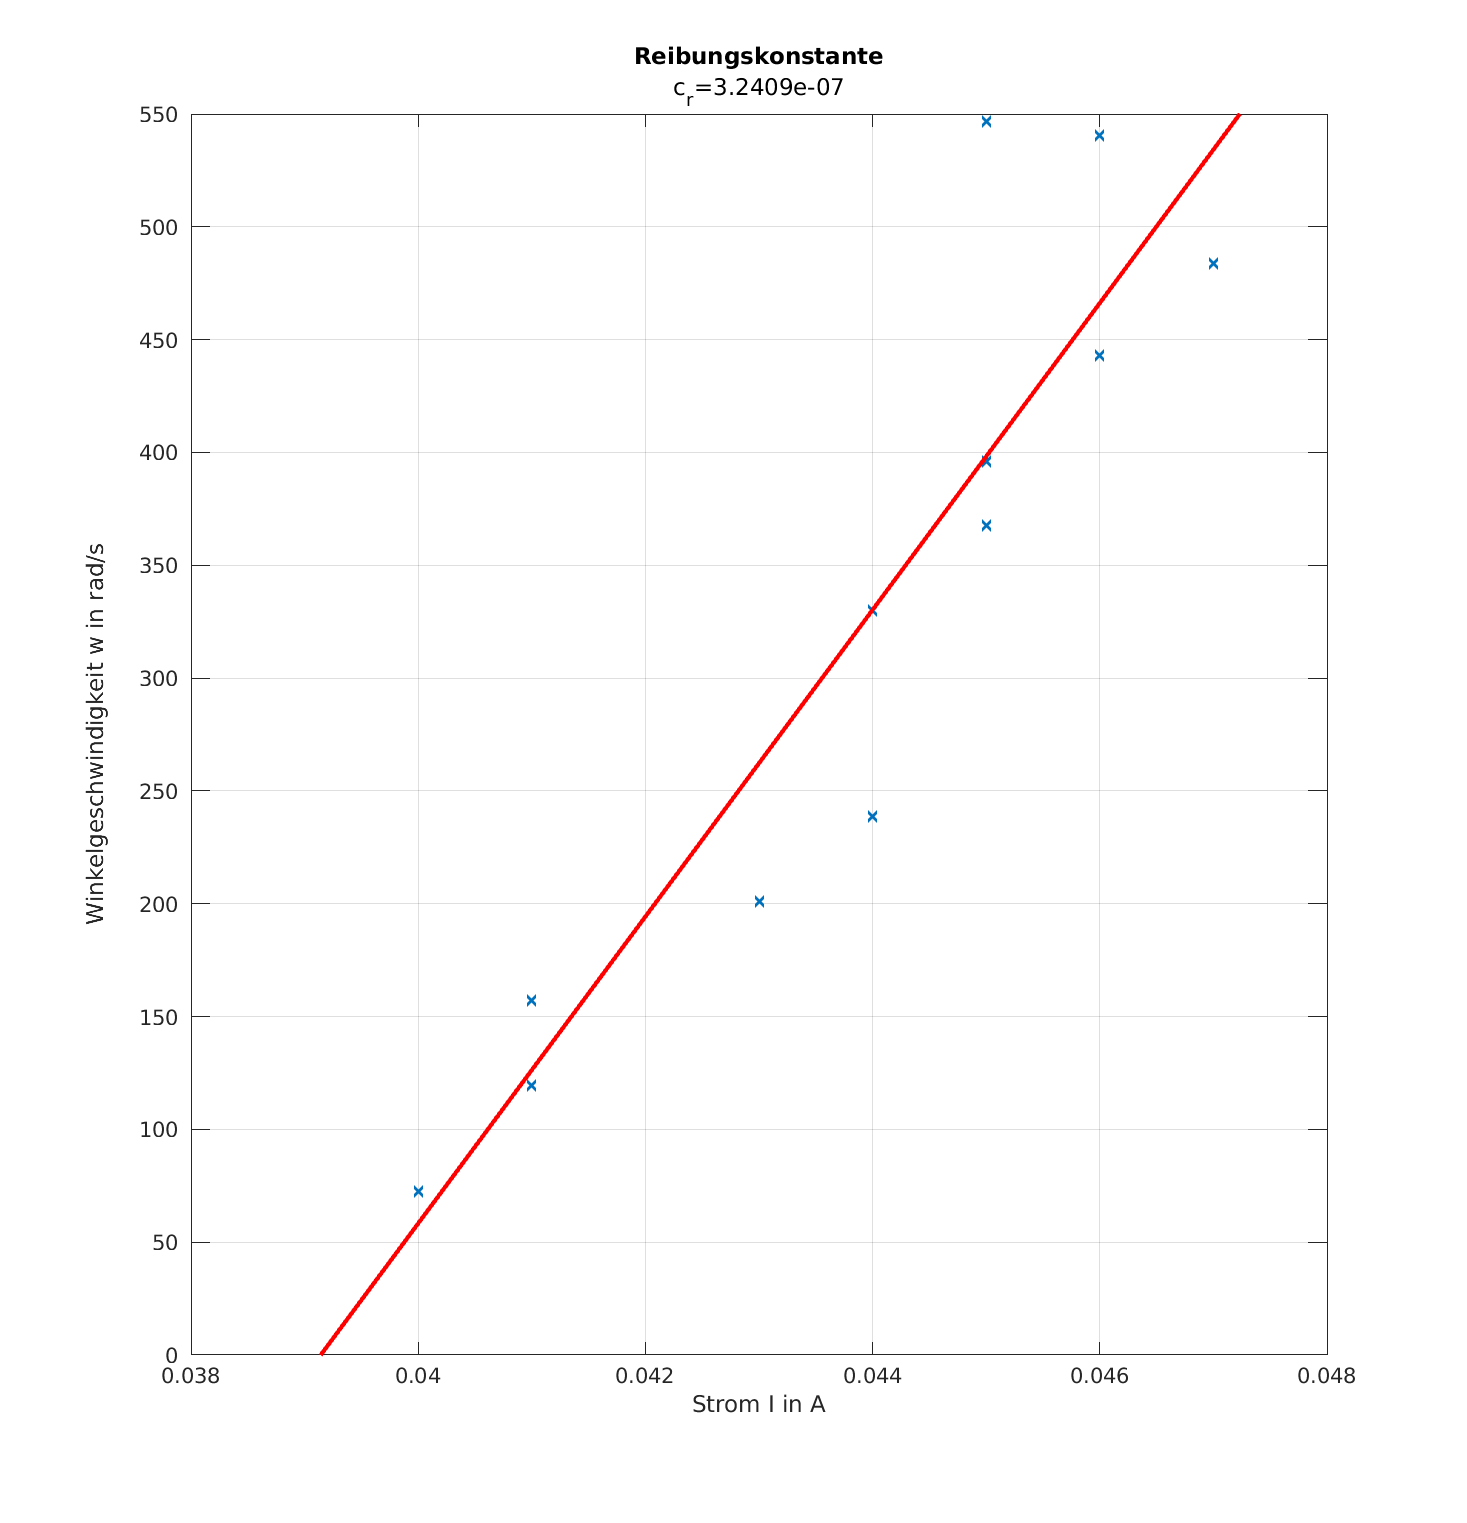
\includegraphics[width=1\textwidth]{as_labor02_2.png}
 \caption{Plot der Aufgabe 1}
 \label{fig:PlotAufgabe1}
\end{figure}